\section{Modalità di esecuzione dei test}
In questa sezione si andrà ad analizzare le performance delle tre soluzioni VPN descritte nei capitoli precedenti, al fine di valutare quale di esse offre le prestazioni migliori.
Le prestazioni verranno valutate analizzando il throughput, la sua stabilità e la percentuale di packetloss.
I software che sono stati utilizzati per effettuare le misurazioni questi dati sono \texttt{iPerf3} e \texttt{mrt}.

\subsection{Panoramica di \texttt{iPerf3}}
\texttt{iPerf} è uno strumento open source che permette di misurare le prestazioni di una rete.
Per effettuare le misurazioni, iPerf crea dei flussi di dati su TCP, UDP o SCTP e invia traffico da un host all'altro; al termine del trasferimento, oltre a un report dettagliato in base al tipo di misurazione richiesta, mostra la larghezza di banda media disponibile.
In questo modo, gli utenti possono determinare il throughput effettivamente utilizzabile.

\begin{figure}[ht]
    \centering
    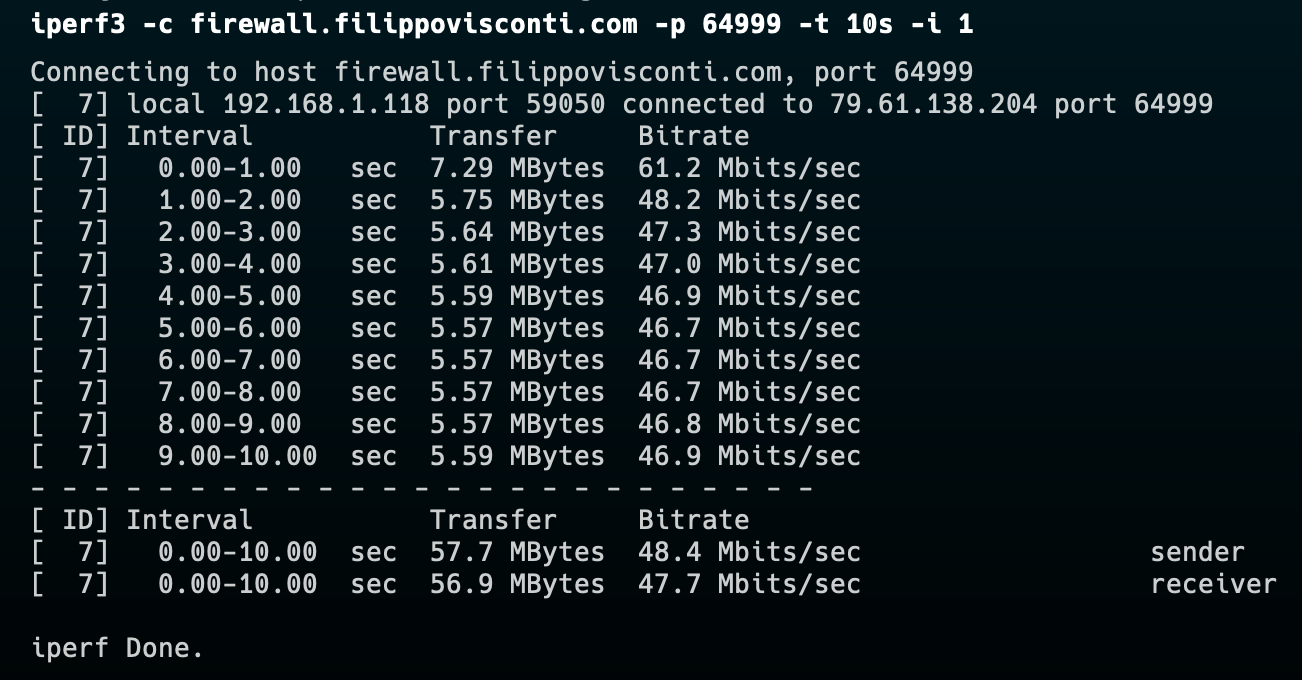
\includegraphics[width=10cm]{figure/iperfSample.png}
    \caption{Esempio di output di iPerf3}
\end{figure}

\subsection{Panoramica di \texttt{mrt}}
\texttt{mtr} è un altro software di misurazione delle performance di una rete, che sostanzialmente unisce i risultati di traceroute e ping.
I test effettuati da mtr sono unidirezionali, dunque è opportuno effettuare misurazioni manualmente in entrambe le direzioni, in quanto i risultati differire in maniera sostanziale. Per avere una misurazione affidabile, è consigliabile far durare il test almeno 10 minuti.


MTR relies on Internet Control Message Protocol (ICMP) Time Exceeded (type 11, code 0) packets coming back from routers, or ICMP Echo Reply packets when the packets have hit their destination host. MTR also has a User Datagram Protocol (UDP) mode (invoked with "-u" on the command line or pressing the "u" key in the curses interface) that sends UDP packets, with the time to live (TTL) field in the IP header increasing by one for each probe sent, toward the destination host. When the UDP mode is used, MTR relies on ICMP port unreachable packets (type 3, code 3) when the destination is reached.

MTR also supports IPv6 and works in a similar manner but instead relies on ICMPv6 messages.

The tool is often used for network troubleshooting. By showing a list of routers traversed, and the average round-trip time as well as packet loss to each router, it allows users to identify links between two given routers responsible for certain fractions of the overall latency or packet loss through the network.[4] This can help identify network overuse problems.[5]

\begin{figure}[ht]
    \centering
    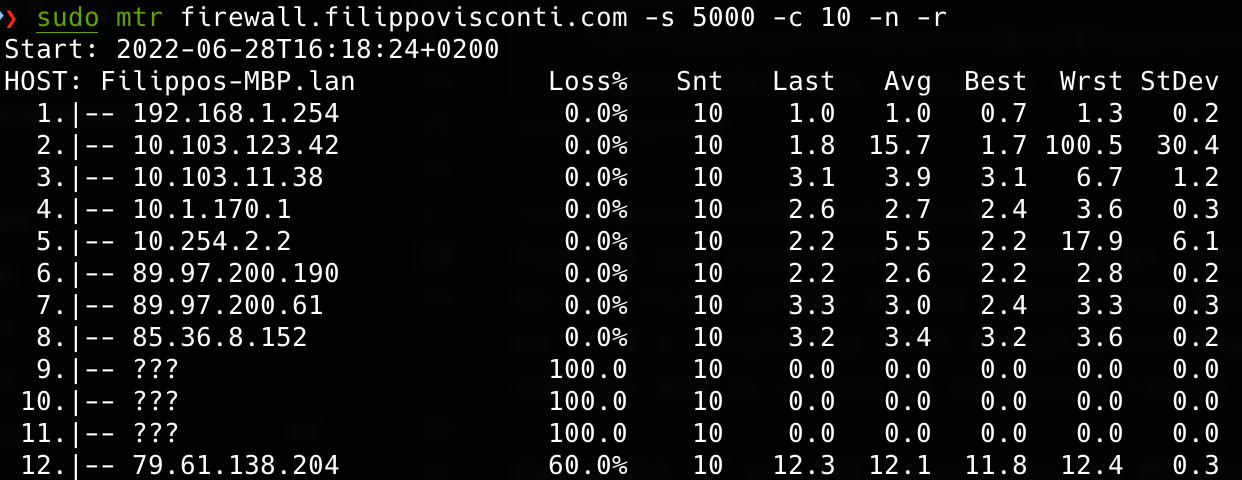
\includegraphics[width=10cm]{figure/mtrSample.png}
    \caption{Esempio di output di mrt}
\end{figure}

\subsubsection{Spiegazione del formato dell'output}
Nella prima colonna, si legge un numero e un indirizzo IP: il numero corrisponde alla distanza in hop tra l'host da cui parte il test e l'IP indicato alla sua destra.
La seconda colonna, \texttt{Loss\%}, indica la percentuale di pacchetti che quell'IP ha perso. È auspicabile un valore inferiore all'1\% per una connessione affidabile.
La terza colonna, \texttt{Snt}, indica il numero di pacchetti inviati a quell'IP.
Le successive 4 colonne indicano il valore dell'ultimo, del medio, del migliore e del peggiore round-trip-time in millisencondi - ossia il tempo necessario affinché un pacchetto parta dal mittente, raggiunga il destinatario, e torni indietro.
L'ultima colonna indica la deviazione standard tra questi ultimi 4 valori.
I valori dalla terza colonna in poi forniscono dunque informazioni sulla latenza della rete. È desiderabile il valore più basso possibile. Tuttavia,  spesso la latenza dipende da fattori esterni alla rete locale.

Nella misurazione di esempio, è stato richiesto l'invio di 10 pacchetti (\texttt{-c 10}) di dimensione 5000 byte (\texttt{-s 5000}).
Per gli hop 9, 10 e 11, si ha un risultato anomalo: nessun IP restituito e 100\% di packet loss.
Questo risultato non mostra problemi di connessione, ma indica semplicemente che l'host non ha risposto alle richieste indirizzate a lui (per i motivi più disparati, da un carico di lavoro troppo altro, a un firewall che fa cadere quel tipo di pacchetto), e che però, visto che l'hop 12 risponde correttamente, ha inoltrato correttamente quelle destinate a chi gli succede.

\subsection{Criteri di valutazione}
Per dare una valutazione complessiva alle tre soluzioni testate, si andranno a tenere in considerazione i seguenti parametri: throughput, percentuale di packet loss per un pacchetto di grandi dimensioni e latenza media.

\subsubsection{Throughput}
Il throughput di un canale di comunicazione misura la quantità di dati che può essere trasferita tra mittente e destinatario in una data unità di tempo. In ambito reti, si è soliti utilizzare come unità di tempo il secondo e come quantità di dati il bit, o suoi multipli (Kbit, Mbit, Gbit).
La velocità e l'affidabilità di trasmissione dei pacchetti sono parametri fondamentali ed è necessario che siano in grado di soddisfare le necessità dell'azienda proprietaria della rete. Packet loss, latenza e jitter influenzano il throughput di una rete, e più sono elevati, più le performance degradano. Minimizzare tutti questi fattori è un punto cardine della progettazione e ottimizzazione di una rete.
La larghezza di banda potrebbe essere confusa con il throughput; è un valore che misura sempre una quantità di bit trasferiti in un'unità di tempo, ma misura il limite massimo teorico, e non quello reale.

È importante sottolineare che una larghezza di banda maggiore non conferisce più velocità, bensì dà soltanto la possibilità di trasferire allo stesso momento una quantità di dati maggiore. Se si hanno problemi di latenza e di perdita dei pacchetti, questi non verranno risolti aumentando la larghezza di banda.


\subsubsection{Packetloss}
Quando un pacchetto non riesce a raggiungere la destinazione prevista, si verifica il fenomeno della perdita di pacchetti, packet loss.
Un utente avverte questo problema come interruzioni della rete, perdita di connettività e una velocità di connessione rallentata.
Le situazioni in cui si soffre maggiormente questo problema sono tutte quelle in cui è richiesta elaborazione di dati in real-time, dove i ritardi non sono tollerati.

Nel caso di una connessione TCP, la perdita di un pacchetto non comporta perdita di dati, in quanto il protocollo è in grado di chiedere la ritrasmissione del pacchetto perduto; tuttavia, ciò comporta comunque un aumento della latenza e una riduzione del throughput generale.

Un pacchetto potrebbe essere scartato anche se, ad esempio, l'IPv4 header checksum o l'Ethernet frame check sequence indicano che il pacchetto è stato corrotto.

La perdita dei pacchetti viene misurata come la percentuale dei pacchetti che una rete ha effettivamente gestito, rispetto a quanti ne avrebbe in teoria dovuto gestire.


\subsubsection{Latenza}
La latenza di una rete, a volte chiamata anche lag, è un termine che descrive i ritardi di comunicazione attraverso una rete. In particolare, si intente il tempo necessario affinché un pacchetto venga catturato, trasmesso, processato attraverso molteplici apparati, ricevuto dal destinatario e decodificato.

La latenza è generalmente misurata in millisecondi. Minore è la latenza, migliori sono le performance. Una latenza inferiore ai 100ms è considerata accettabile, ma per buone performace si desidera un valore inferiore ai 40ms. Ovviamente, un valore prossimo agli 0ms sarebbe ideale.

\subsection{Scelta della configurazione di test}
Per effettuare i test, sono stati scelti i seguenti parametri:


\texttt{iperf3 -c [IP ADDRESS] -p 5201 -t 300s -i 5}


Si effettuerà un test lungo 300 secondi, con report ogni 5 secondi.

\texttt{mtr [IP ADDRESS] -s 5000 -c 1000}


Si invi

\section{Misure senza VPN}
\begin{figure}[ht]
    \centering
    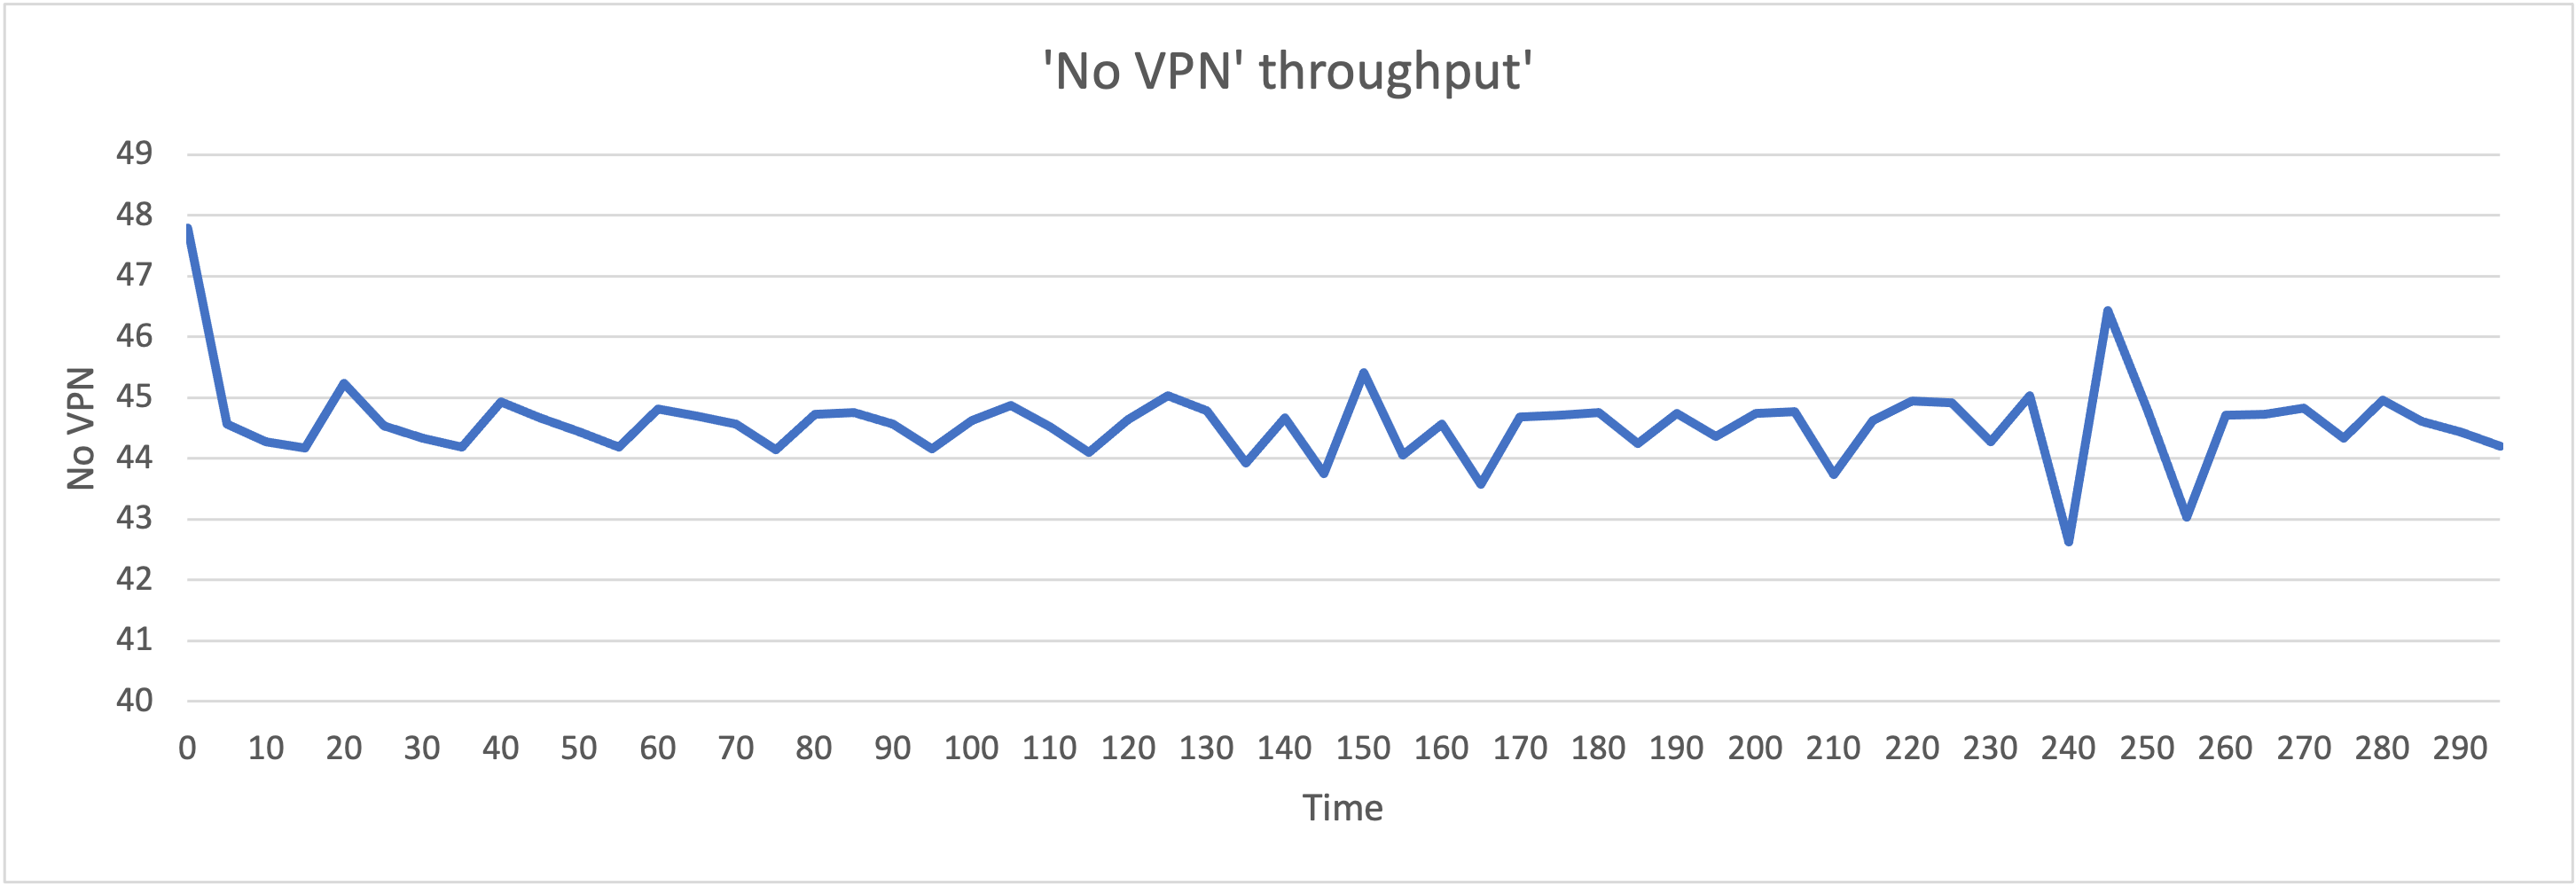
\includegraphics[width=12cm]{figure/vpn_thr.png-1.png}
    \caption{Throughput senza VPN su 300 secondi}
\end{figure}
Nella configurazione base, senza VPN, si può osservare come il throughput sia stabile tra i 44 e i 45 Mbit/s, eccetto per i primi istanti, dovuti ad un periodo di assestamento.

\begin{figure}[ht]
    \centering
    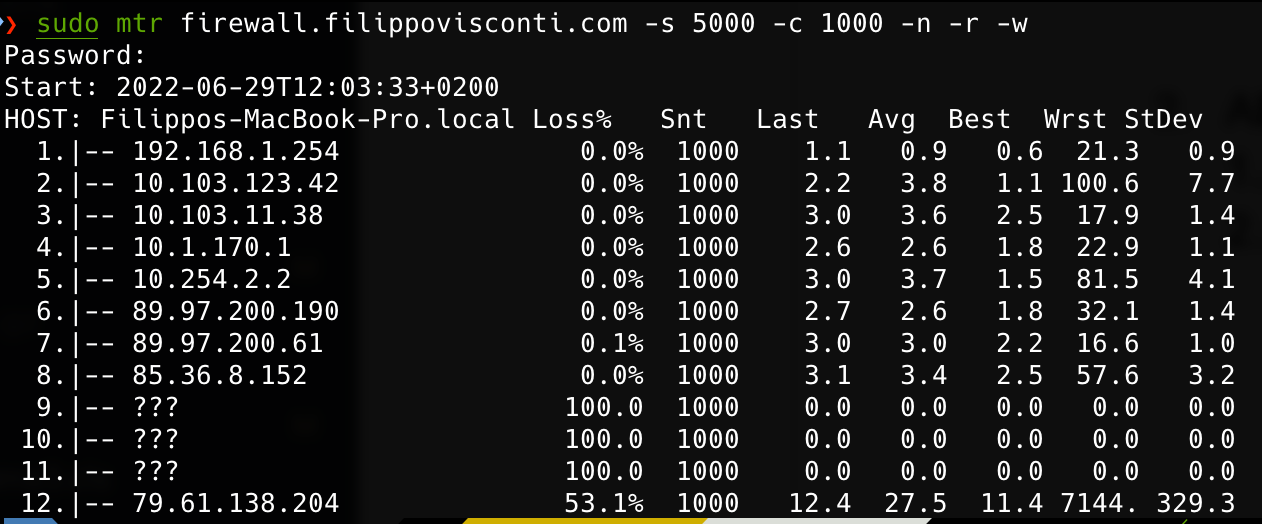
\includegraphics[width=10cm]{figure/mrt_16min_noVPN.png}
    \caption{mrt senza VPN}
\end{figure}

In questo grafico invece, si può notare come, fino all'ottavo hop, la latenza sia generalmente bassa e la percentuale di packet loss irrisoria. Gli hop 9, 10 e 11 non rispondono, ma ciò non vuol dire che non funzionino. L'ultimo hop, quello del router di destinazione, ha una percentuale di packetloss molto elevata (più del 50\%) e una latenza più elevata, seppur ancora accettabile.

\section{Misure con IPSec e IKEv2}
\begin{figure}[ht]
    \centering
    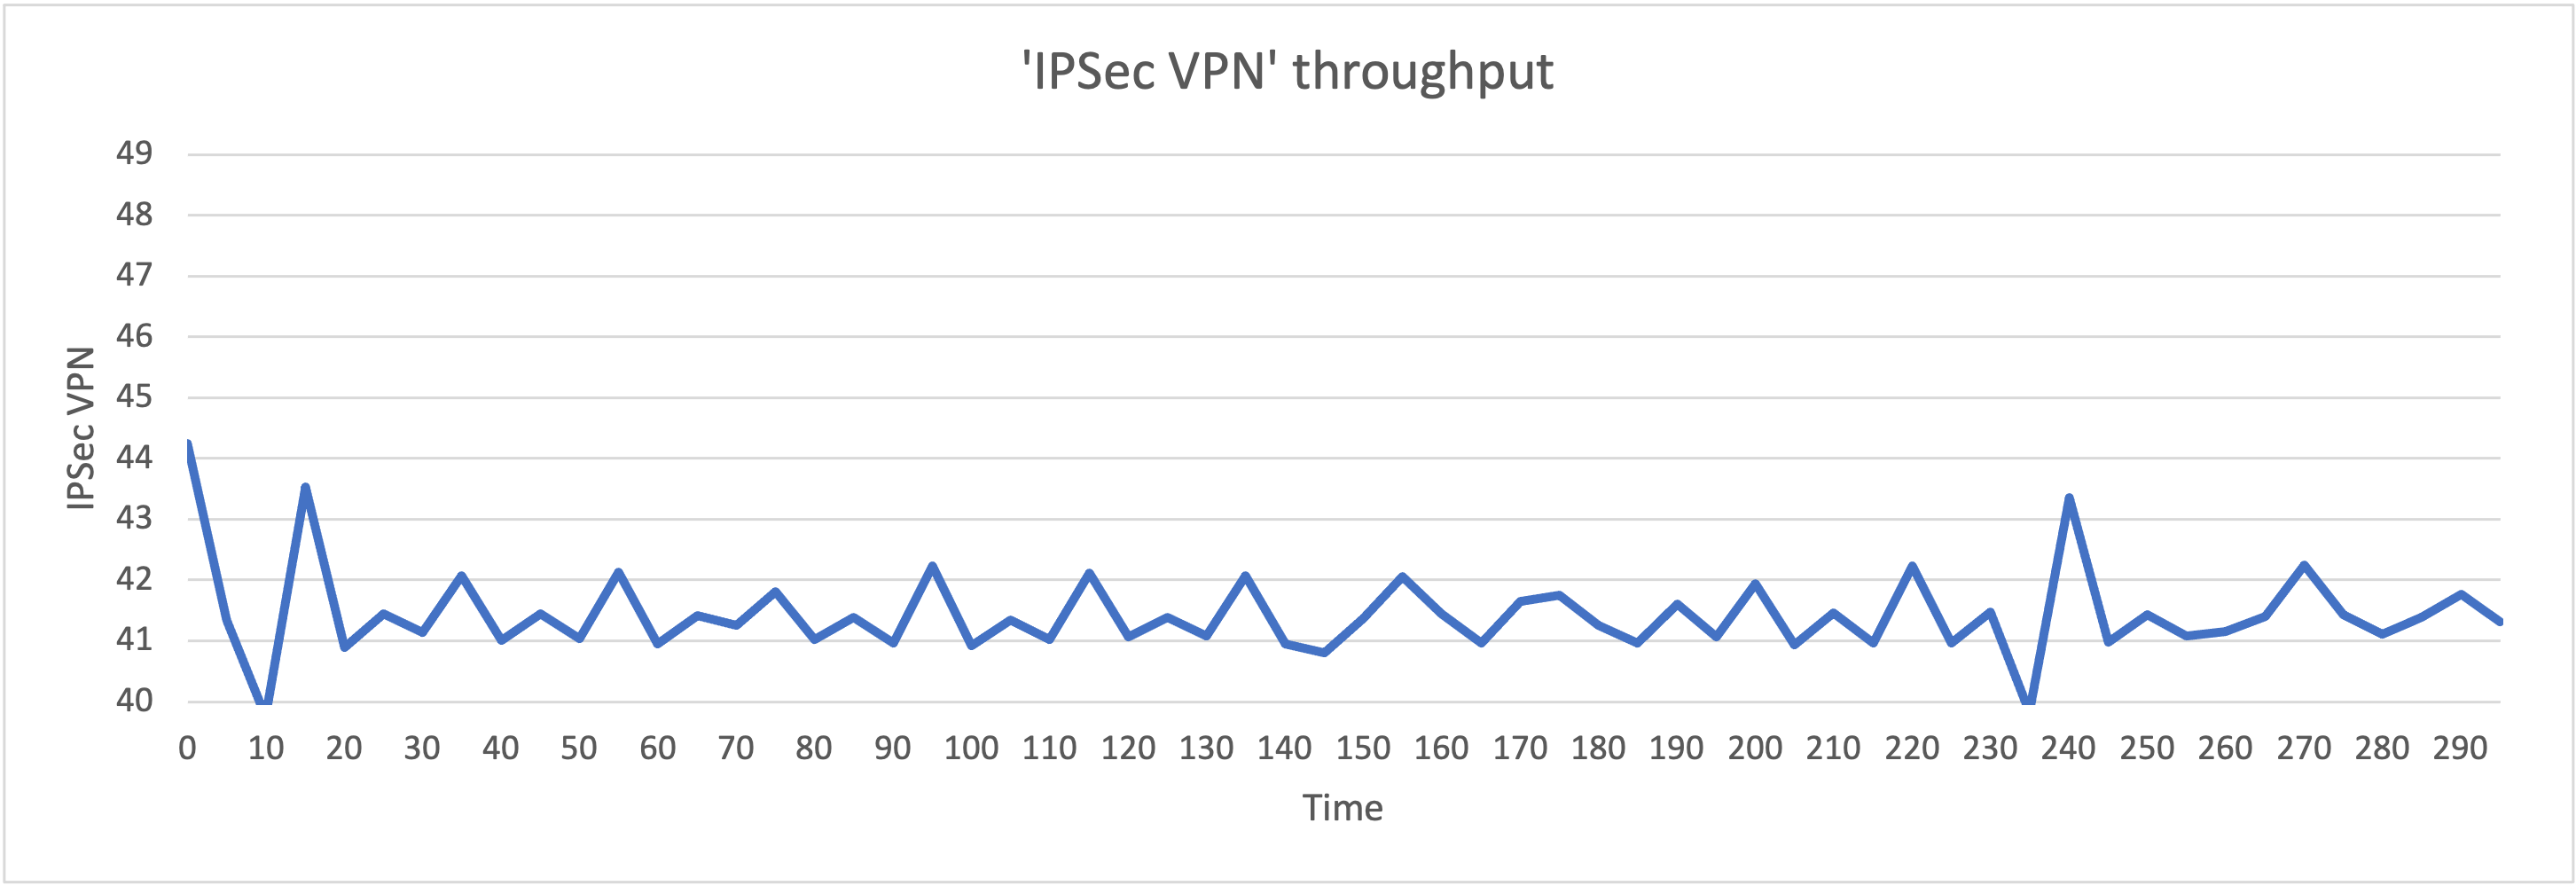
\includegraphics[width=12cm]{figure/vpn_thr.png-2.png}
    \caption{IPSec Throughput su 300 secondi}
\end{figure}
Ripetendo lo stesso test attraverso un tunnel IPSec, si nota come il throughput sia calato e oscilli tra i 41 e i 42 Mbit/s.

\begin{figure}[ht]
    \centering
    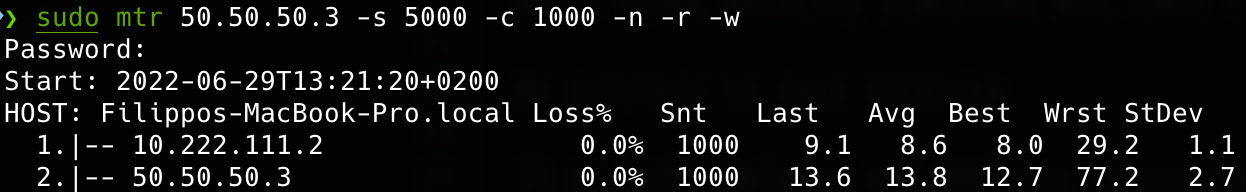
\includegraphics[width=10cm]{figure/mtr_16min_ipsec.png}
    \caption{mrt su IPSec}
\end{figure}
Il secondo test invece riporta una packetloss a destinazione nulla, ossia nessun pacchetto è stato perso, e una latenza media migliore rispetto a quella del test precedente.


\section{Misure con OpenVPN over TCP}
\begin{figure}[ht]
    \centering
    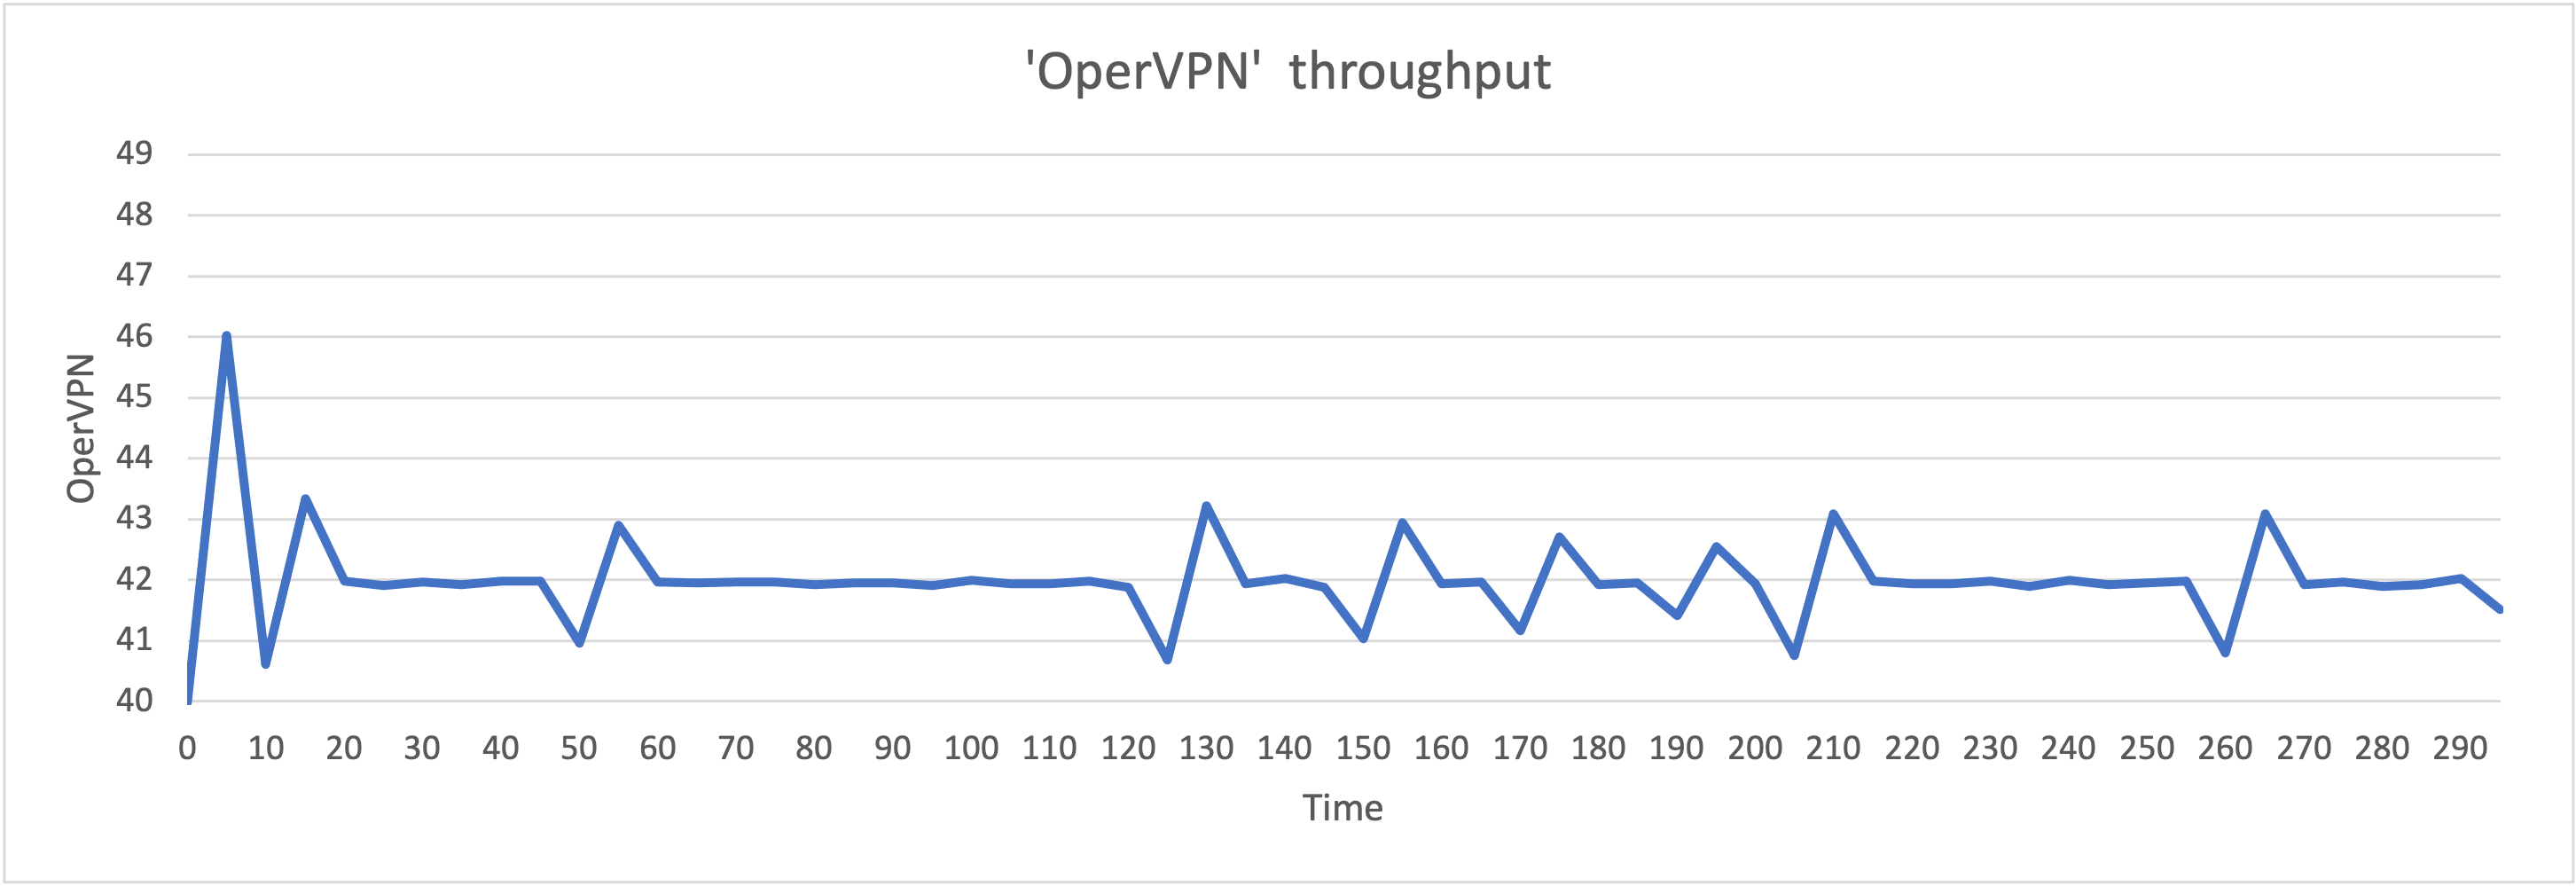
\includegraphics[width=12cm]{figure/vpn_thr.png-3.png}
    \caption{OpenVPN Throughput su 300 secondi}
\end{figure}
Con OpenVPN, il primo test registra un throughput medio marginalmente più alto di IPSec, anche se con oscillazioni leggermente più ampie.

\begin{figure}[ht]
    \centering
    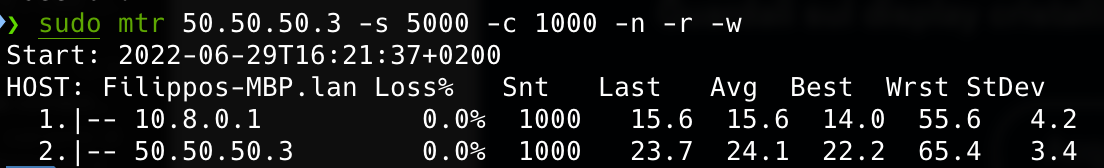
\includegraphics[width=10cm]{figure/mtr_16min_ovpn.png}
    \caption{mrt su OpenVPN}
\end{figure}
Nel secondo test, si ha ugualmente lo 0\% di packetloss, ma una latenza media maggiore di 10ms; si tratta comunque di un valore ampiamente accettabile.


\section{Misure con WireGuard}
\begin{figure}[ht]
    \centering
    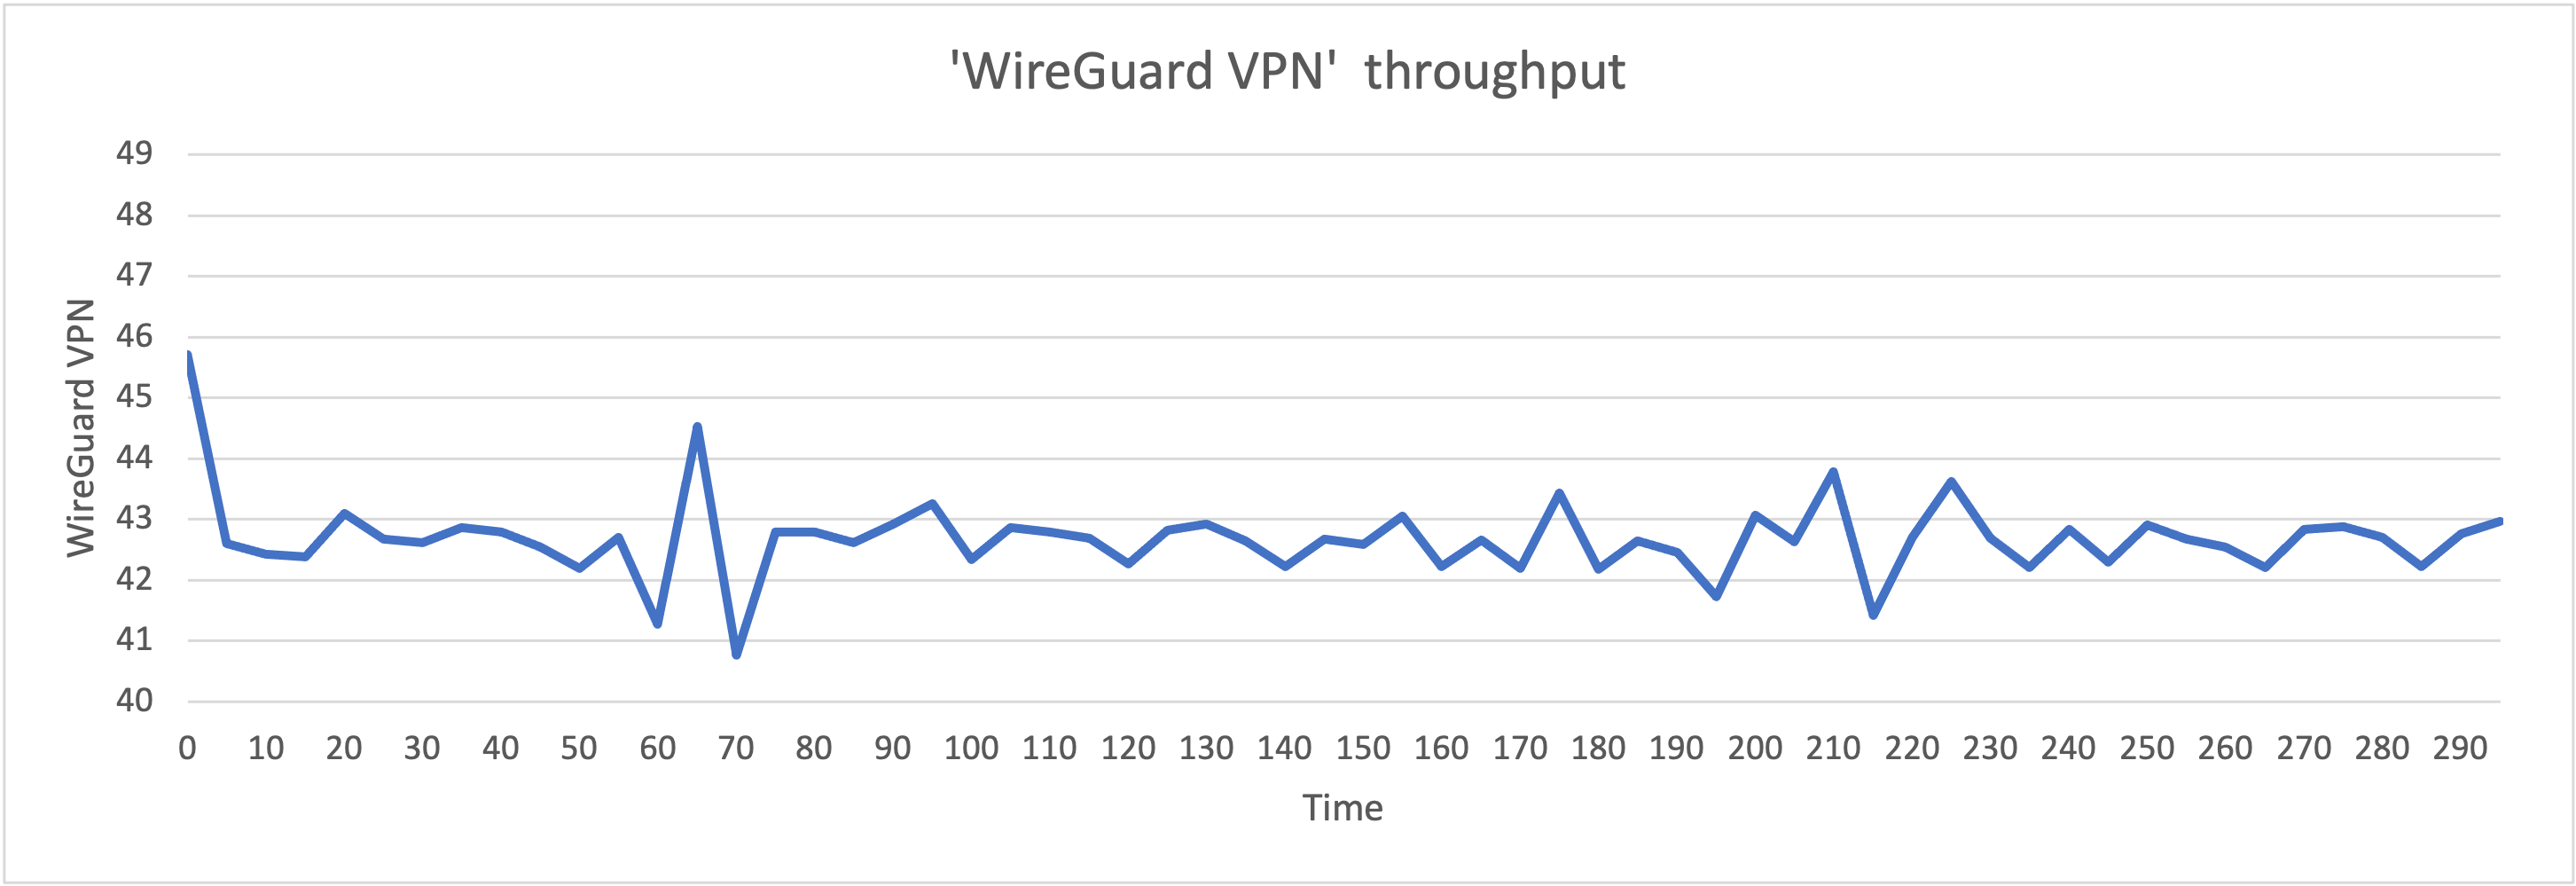
\includegraphics[width=12cm]{figure/vpn_thr.png-4.png}
    \caption{WireGuard Throughput su 300 secondi}
\end{figure}
Utilizzando WireGuard, nel primo test si raggiunge il risultato migliore, con un throughput medio che sfiora i 43 Mbit/s.

\begin{figure}[ht]
    \centering
    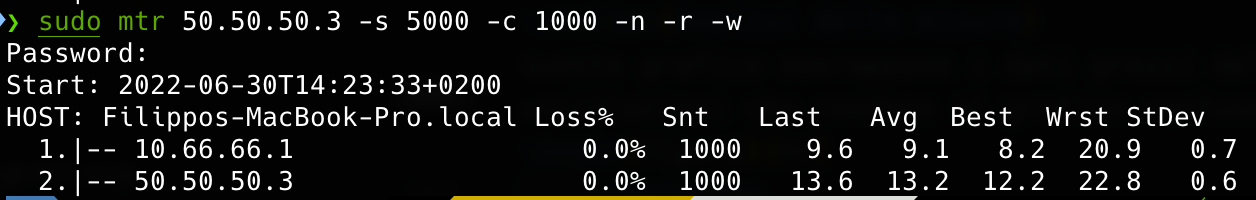
\includegraphics[width=10cm]{figure/mrt_16min_wg.png}
    \caption{mrt su WireGuard}
\end{figure}

Nel secondo test, come nelle altre soluzioni VPN, la percentuale di packetloss è a 0, e la latenza è pari a quella ottenuta tramite la soluzione con IPSec, dunque molto buona.

\section{Analisi delle misure}
Questo grafico sovrappone i dati grezzi del primo test, riguardante il throughput medio. Essendo campionato ogni secondo, sono presenti molte oscillazioni che rendono il grafico confuso.
\begin{figure}[ht]
    \centering
    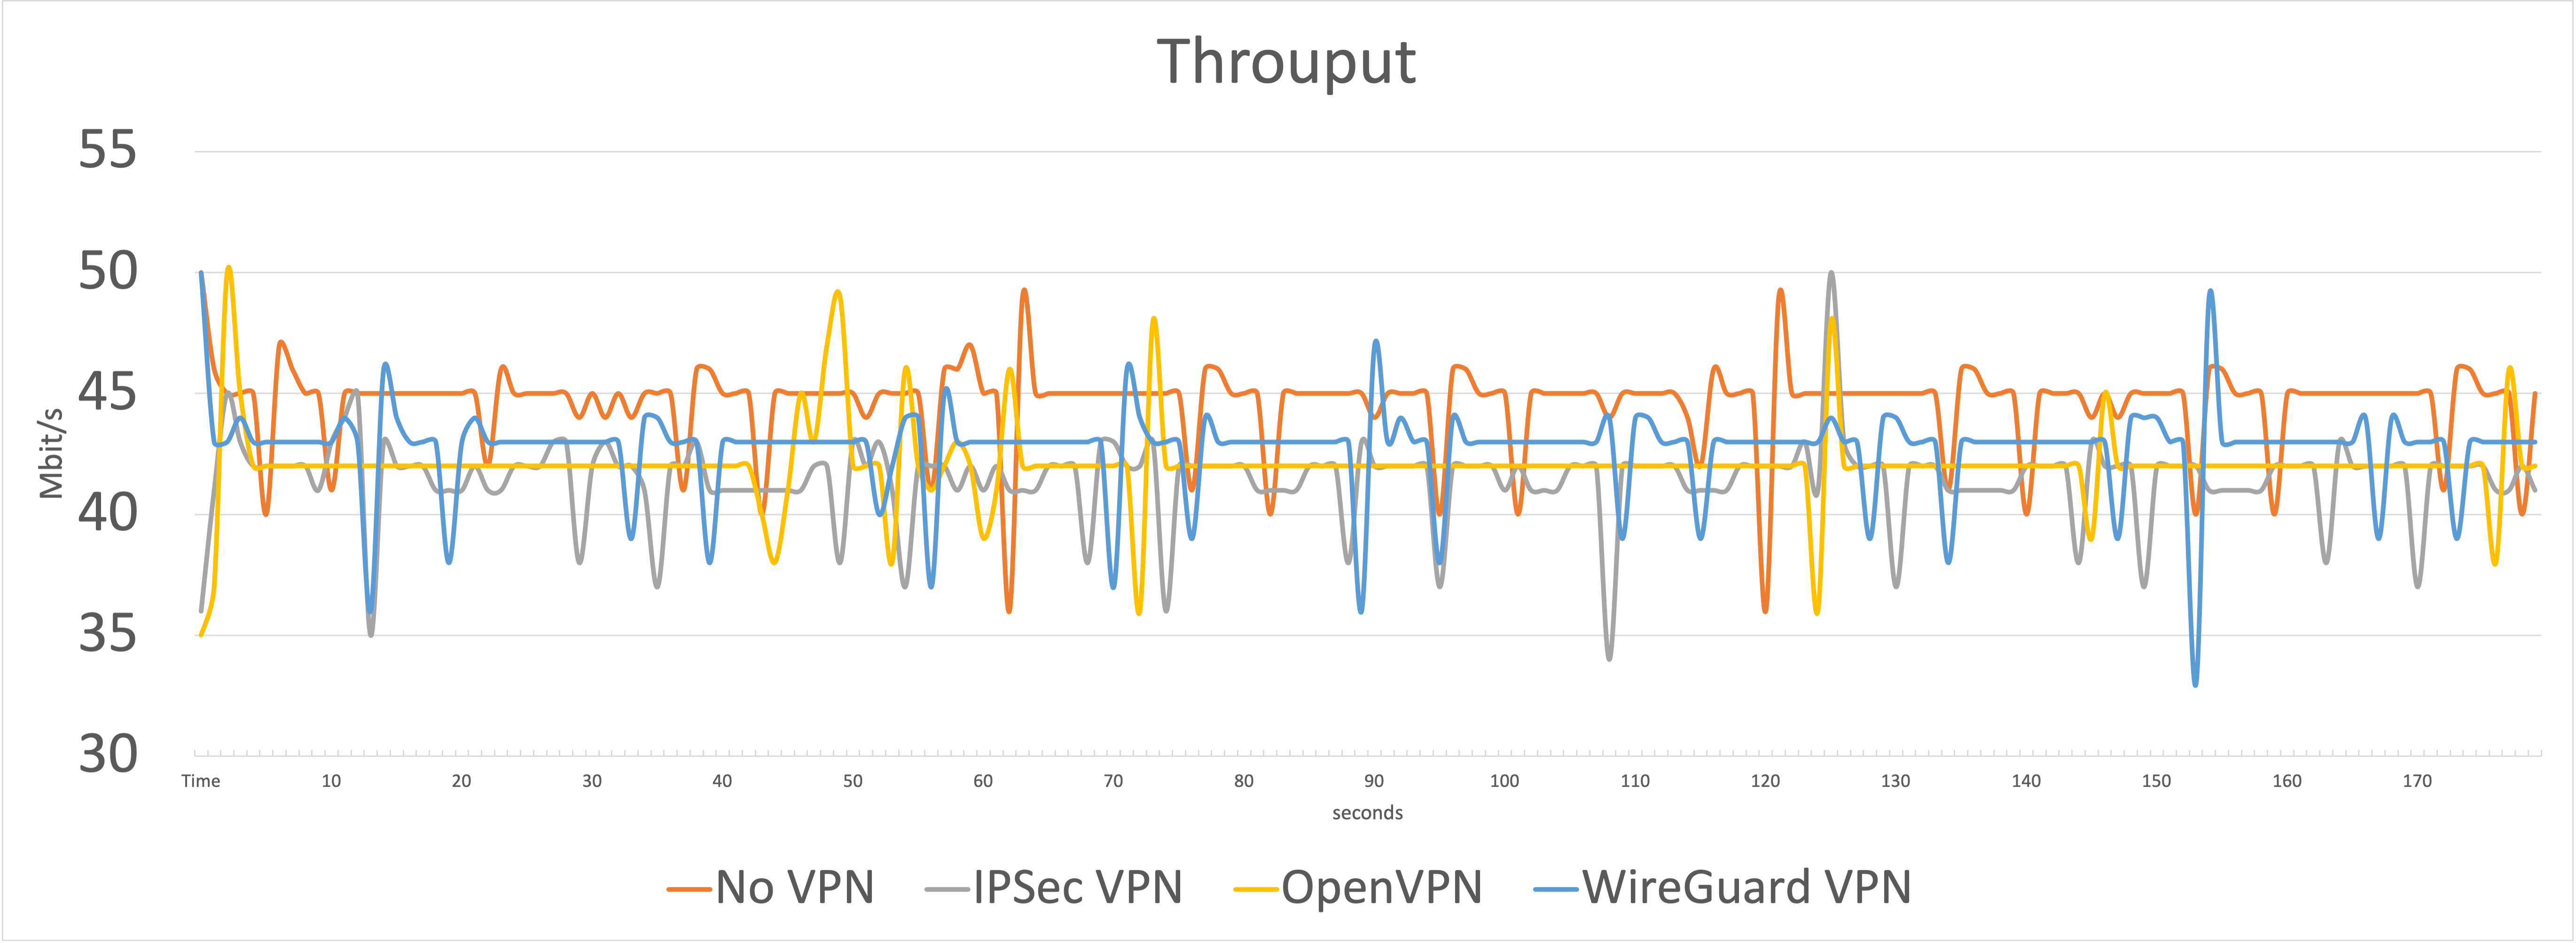
\includegraphics[width=14cm]{figure/rawThroughput.png}
    \caption{Confronto dei throughput grezzi}
\end{figure}

Campionando invece ogni 5 secondi, si riducono le oscillazioni, che essendo di lieve entità sono poco significative, e diventa chiara la classifica di performance in termini di throughput tra i 4 casi.


\begin{figure}[ht]
    \centering
    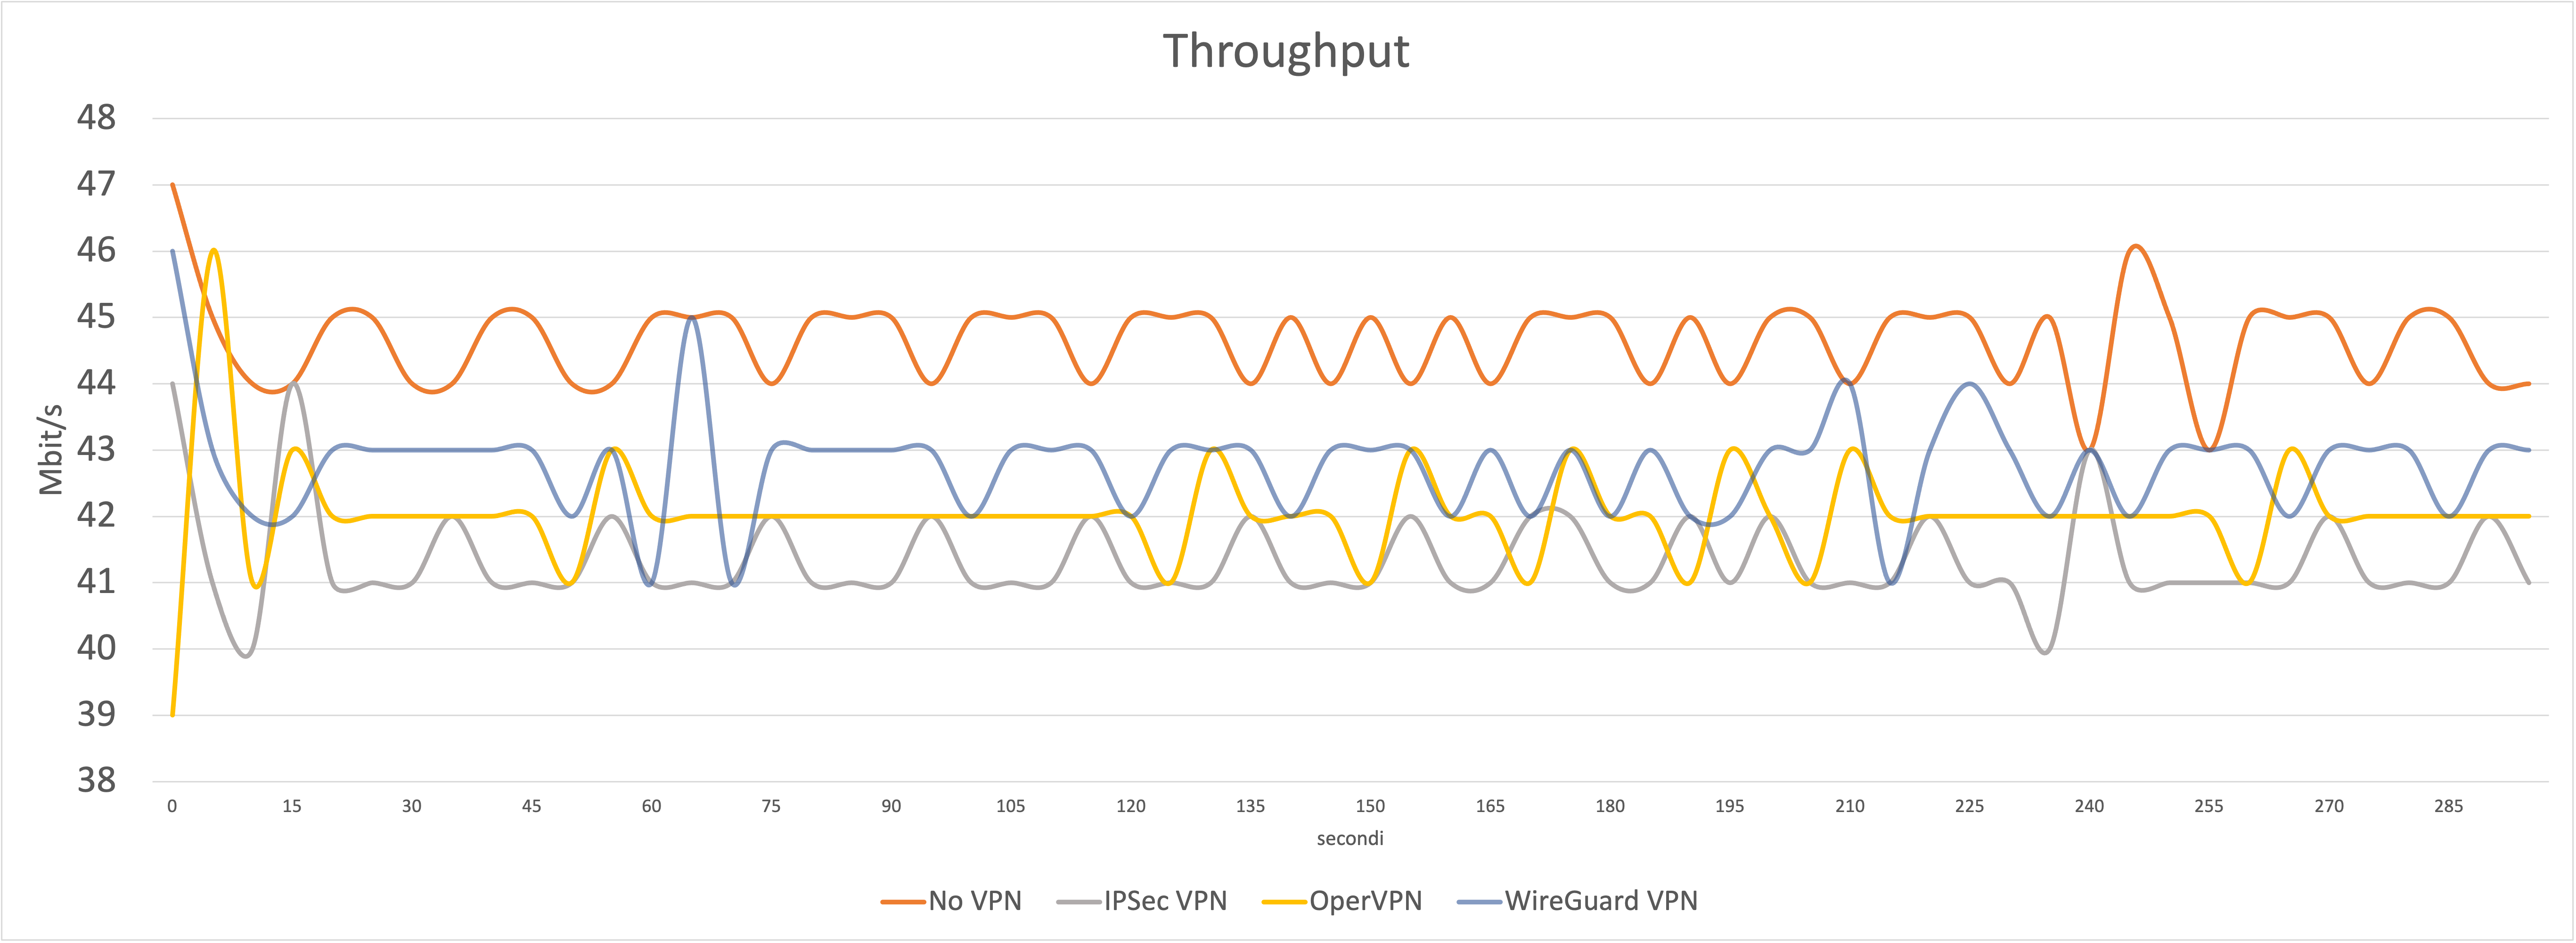
\includegraphics[width=14cm]{figure/fineThroughput.png}
    \caption{Confronto dei throughput raffinati}
\end{figure}
In questo caso, escluso il caso senza VPN che ovviamente utilizza tutta la banda disponibile per trasferire dati, la soluzione più performante è WireGuard, seguita da OpenVPN e IPSec

\begin{figure}[ht]
    \centering
    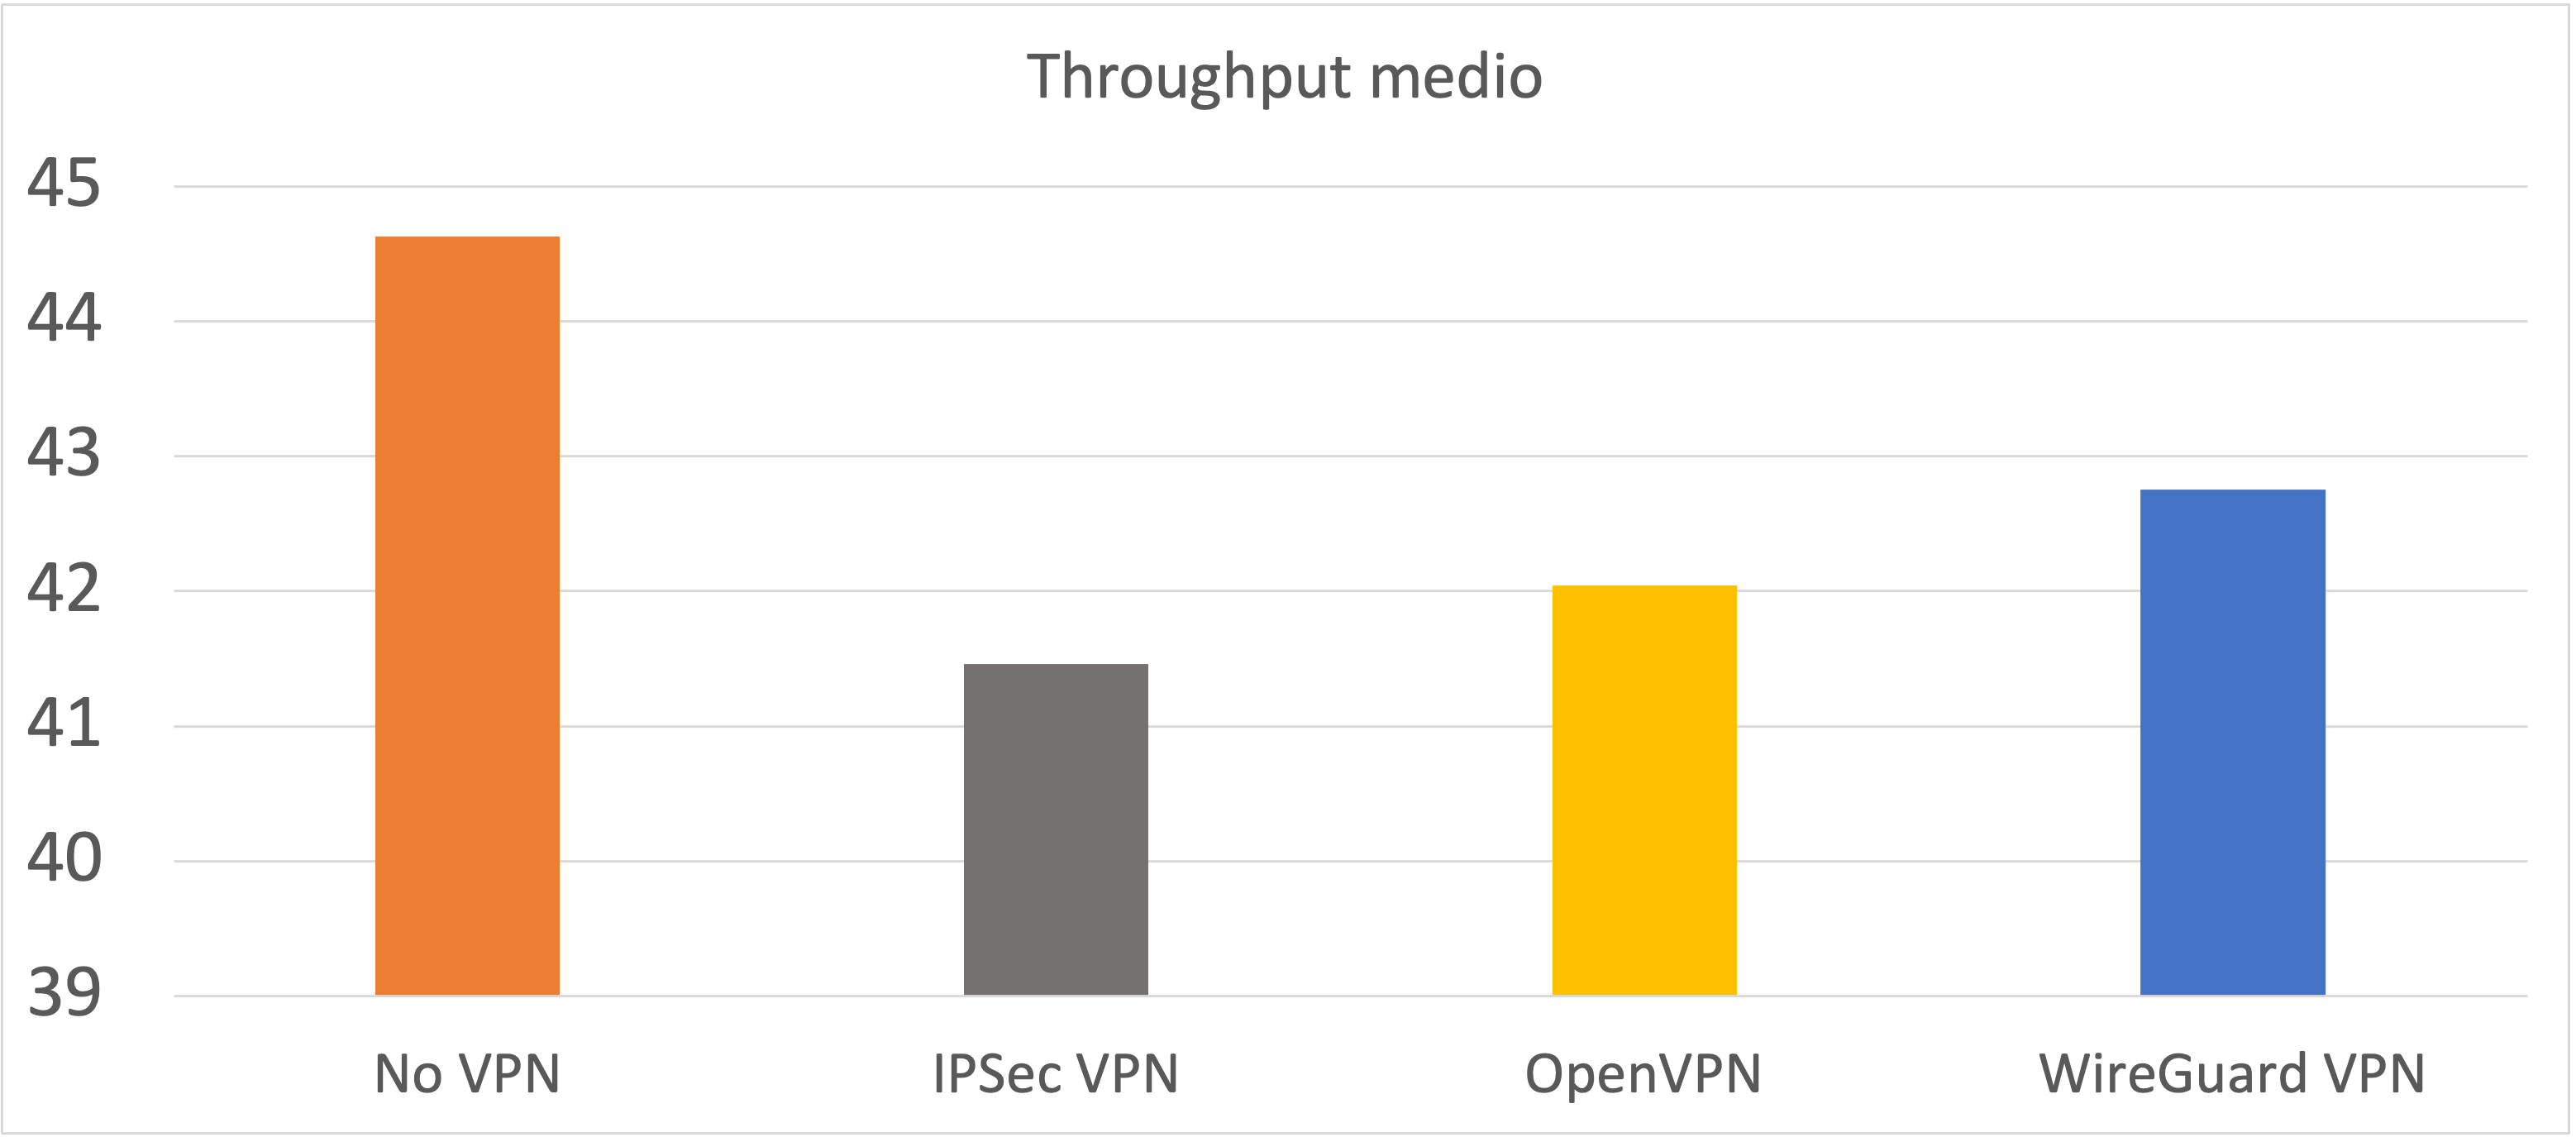
\includegraphics[width=10cm]{figure/avg.png}
    \caption{Confronto dei throughput medi}
\end{figure}